% GEST-2026 Poster — Shen Ruililin
% Single-page A0 landscape with absolute positioning
\documentclass[10pt]{article}
\usepackage[margin=0pt,paperwidth=118.9cm,paperheight=84.1cm]{geometry}
\usepackage[T1]{fontenc}
\usepackage[utf8]{inputenc}
\usepackage{lmodern}
\usepackage{graphicx}
\usepackage{booktabs}
\usepackage{tabularx}
\usepackage{array}
\usepackage{xcolor}
\usepackage{enumitem}
\usepackage{microtype}
\usepackage{ragged2e}
\usepackage[absolute,overlay]{textpos}
\usepackage{tcolorbox}
\tcbuselibrary{skins,breakable}

\pagestyle{empty}
\setlength{\parindent}{0pt}
\setlength{\parskip}{0.2em}
\setlength{\TPHorizModule}{1cm}
\setlength{\TPVertModule}{1cm}
\textblockorigin{0cm}{0cm}
\setlist[itemize]{leftmargin=1.05em,itemsep=0.12em,topsep=0.15em,parsep=0pt}
\setlist[enumerate]{leftmargin=1.2em,itemsep=0.15em,topsep=0.15em,parsep=0pt}

\definecolor{Ink}{HTML}{1A2332}
\definecolor{Teal}{HTML}{0B5B6B}
\definecolor{TealDark}{HTML}{083F4A}
\definecolor{TealSoft}{HTML}{E6F2F4}
\definecolor{Muted}{HTML}{5A6570}
\definecolor{Panel}{HTML}{F7FAFB}
\definecolor{Warn}{HTML}{8B4513}
\color{Ink}

\newcommand{\posterbox}[2]{%
  \begin{tcolorbox}[
    enhanced,
    colback=Panel,
    colframe=Teal,
    boxrule=1.0pt,
    arc=2pt,
    left=9pt,right=9pt,top=7pt,bottom=7pt,
    coltitle=white,
    fonttitle=\bfseries\fontsize{15}{18}\selectfont,
    attach boxed title to top left={yshift=-2mm,xshift=5mm},
    boxed title style={
      colback=Teal,colframe=Teal,arc=1.5pt,boxrule=0pt,
      left=7pt,right=7pt,top=2pt,bottom=2pt
    },
    title={{#1}},
    before skip=0pt,
    after skip=0.28cm,
    width=\linewidth
  ]
  \RaggedRight\fontsize{11.5}{14.2}\selectfont #2
  \end{tcolorbox}%
}

\newcommand{\statchip}[2]{%
  \begin{tcolorbox}[
    enhanced,width=\linewidth,
    colback=TealSoft,colframe=Teal,boxrule=0.7pt,arc=1.5pt,
    left=5pt,right=5pt,top=3pt,bottom=3pt,
    before skip=0.08cm, after skip=0.08cm
  ]
  {\centering\color{Teal}\bfseries\fontsize{16}{18}\selectfont #1\par}
  {\centering\color{Muted}\fontsize{9}{11}\selectfont #2\par}
  \end{tcolorbox}%
}

\emergencystretch=3em
\begin{document}

% HEADER
\begin{textblock*}{115.3cm}(1.8cm,1.2cm)
\begin{tcolorbox}[
  enhanced,colback=TealDark,colframe=TealDark,boxrule=0pt,arc=0pt,
  left=12pt,right=12pt,top=7pt,bottom=6pt,width=\linewidth
]
  \textcolor{white}{\bfseries\fontsize{26}{30}\selectfont
  Rising hot nights, persistent cold days, and an aging population:}\\[1pt]
  \textcolor{white}{\bfseries\fontsize{15.5}{18}\selectfont
  thermal extremes and cardiovascular hospital burden in Hong Kong, 2013--2023}\\[3pt]
  \textcolor{TealSoft}{\fontsize{11.5}{14}\selectfont
  Shen Ruililin$^{\ast}$
  \quad\textbar\quad
  BASc (Global Health and Development), School of Public Health, The University of Hong Kong
  \quad\textbar\quad GEST-2026 Poster
  \quad\textbar\quad Environmental Toxicology and Human Health}\\[1pt]
  \textcolor{TealSoft}{\fontsize{10}{12}\selectfont
  Email: shenrll@connect.hku.hk
  \quad$\cdot$\quad Laidlaw Scholars research project
  \quad$\cdot$\quad Ecological time-series (exposures \& denominators complete; HA outcomes pending)}
\end{tcolorbox}
\end{textblock*}

% COLUMN 1
\begin{textblock*}{36.5cm}(1.8cm,8.0cm)
\begin{minipage}[t]{36.5cm}
\posterbox{1. Why this matters for human health}{%
Climate change is already reshaping thermal exposure in subtropical cities.
Overnight heat and daytime extremes can impair physiological recovery, while cold snaps
continue to stress cardiovascular systems via blood pressure, viscosity, and autonomic tone.

Earlier local daily studies (e.g.\ Goggins and colleagues) found a
\textbf{cold-dominant} cardiovascular hospitalization profile.
Whether contemporary heat---especially official \textbf{hot nights}
(Tmin\,$\geq$\,28$^\circ$C)---now coexists with persistent cold risk in an
\textbf{aging} population is the open human-health question.
\begin{itemize}
  \item Dense, humid urban living $\rightarrow$ limited overnight cooling
  \item Ages 65--74 nearly doubled (2013--2023) $\rightarrow$ more vulnerable person-time
  \item Hospital burden, not only mortality, matters for adaptation planning
\end{itemize}
}

\posterbox{2. Research aim}{%
\textbf{Aim.} Quantify official thermal extremes and population aging (2013--2023)
as the climate--human exposure base for a planned ecological assessment of HA admissions
for AMI, ischemic stroke, and hemorrhagic stroke among residents aged 35+.

\textbf{Design.} Monthly ecological time-series ($N=132$ months); population-level associations only.

\textbf{Framing.} Coexistence of emerging heat with persistent cold---not an assumed heat-for-cold shift.
}

\posterbox{3. Data \& exposure definitions}{%
\renewcommand{\arraystretch}{1.08}
\begin{tabularx}{\linewidth}{@{}l>{\RaggedRight\arraybackslash}X@{}}
\toprule
\textbf{Domain} & \textbf{Source / status} \\
\midrule
Weather & HKO Headquarters daily extracts \textbf{(REAL)} \\
Population & C\&SD Table 110-01001 mid-year age$\times$sex \textbf{(REAL)} \\
Pollution & EPD series (import ready; staged) \\
Outcomes & HA CVD admissions \textbf{(pending HPC access)} \\
\bottomrule
\end{tabularx}
\vspace{0.2em}
\textbf{Official HKO extremes:} hot night Tmin\,$\geq$\,28$^\circ$C;
very hot day Tmax\,$\geq$\,33$^\circ$C;
extremely hot day Tmax\,$\geq$\,35$^\circ$C;
cold day Tmin\,$\leq$\,12$^\circ$C.
Primary heat = monthly hot nights; co-primary cold = monthly cold days.
Validation: annual totals \textbf{33/33 MATCH} vs HKO \textit{Year's Weather}.
}
\end{minipage}
\end{textblock*}

% COLUMN 2
\begin{textblock*}{40.0cm}(39.3cm,8.0cm)
\begin{minipage}[t]{40.0cm}
\posterbox{4. Rising heat, persistent cold (REAL)}{%
\centering
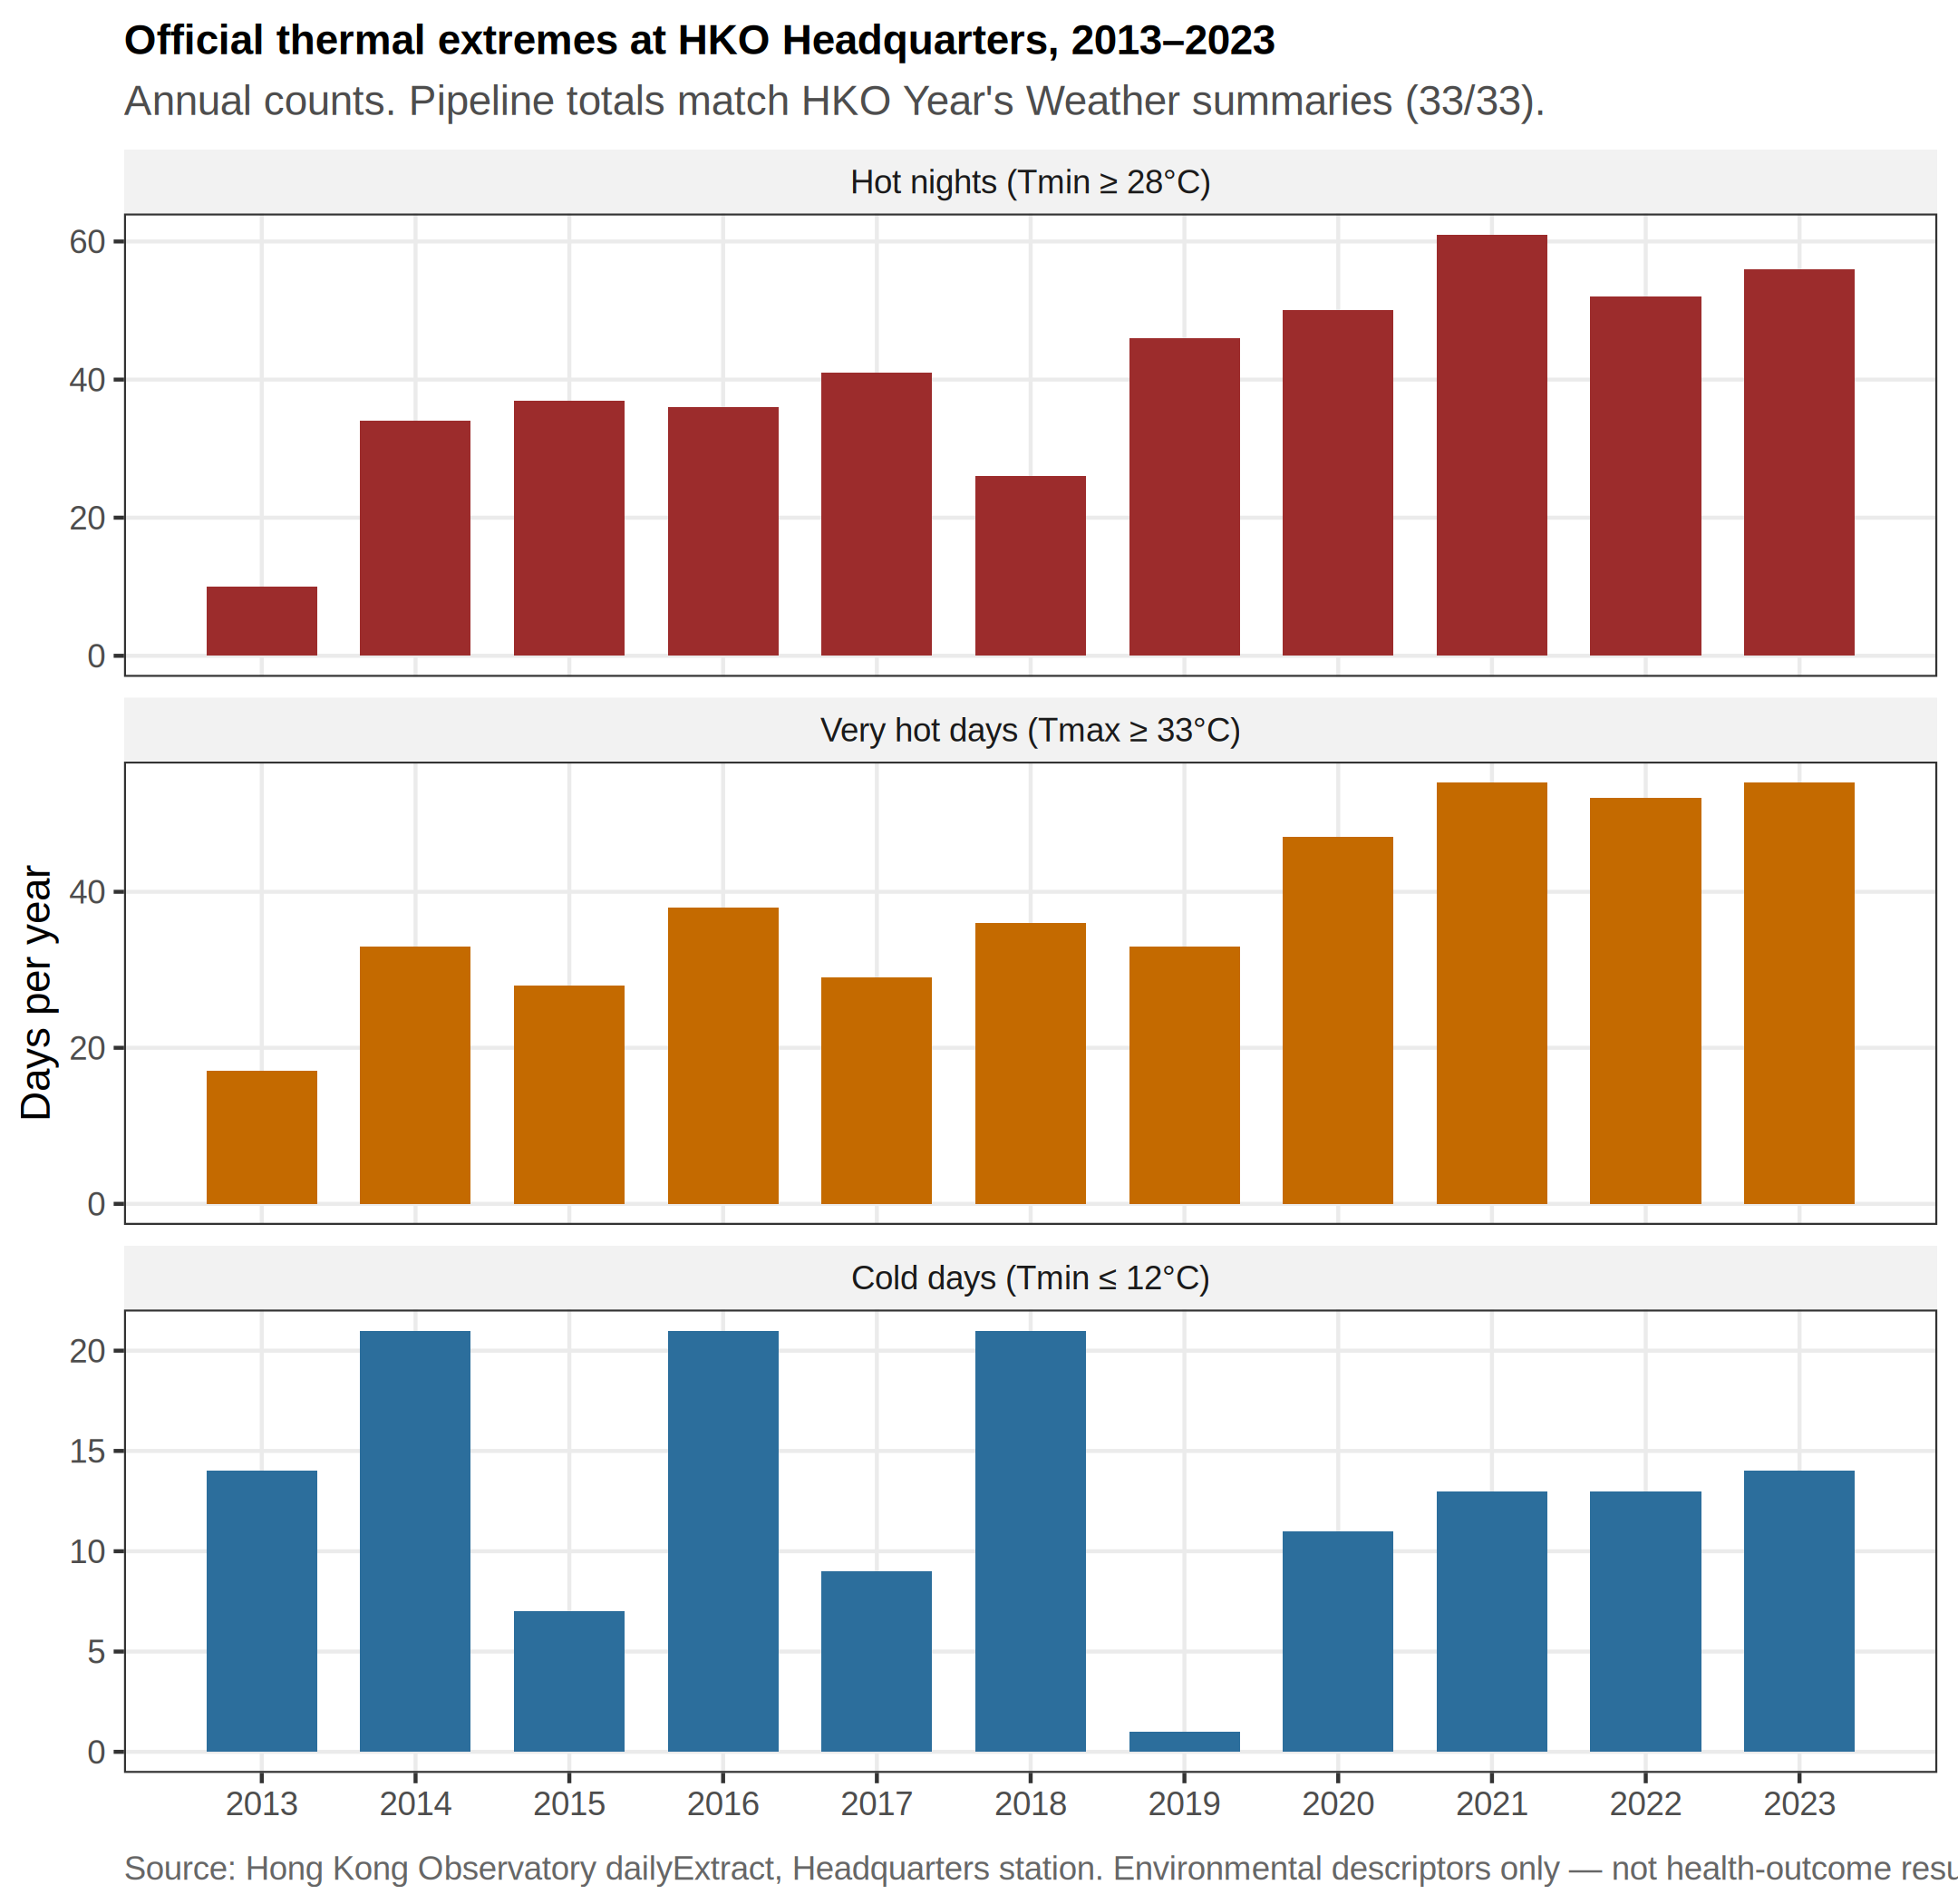
\includegraphics[width=\linewidth,height=18.5cm,keepaspectratio]{../../figures/exposure_aging/fig01_annual_extremes_coexistence.png}\\[1pt]
{\color{Muted}\fontsize{9}{10.5}\selectfont Environmental descriptors only---not health-outcome results.\par}
\begin{flushleft}
\begin{itemize}
  \item Hot nights: \textbf{10 (2013)} $\rightarrow$ \textbf{61 (2021)} / \textbf{56 (2023)}
  \item Period means: \textbf{30.7 $\rightarrow$ 53.0} hot nights/year (2013--18 vs 2019--23)
  \item Cold days persist: \textbf{13--14} days/year in 2021--2023
  \item Hot nights in $\geq$5-night spells: 34\% $\rightarrow$ 51\%
\end{itemize}
\end{flushleft}
}

\posterbox{5. Aging raises the human stakes (REAL)}{%
\centering
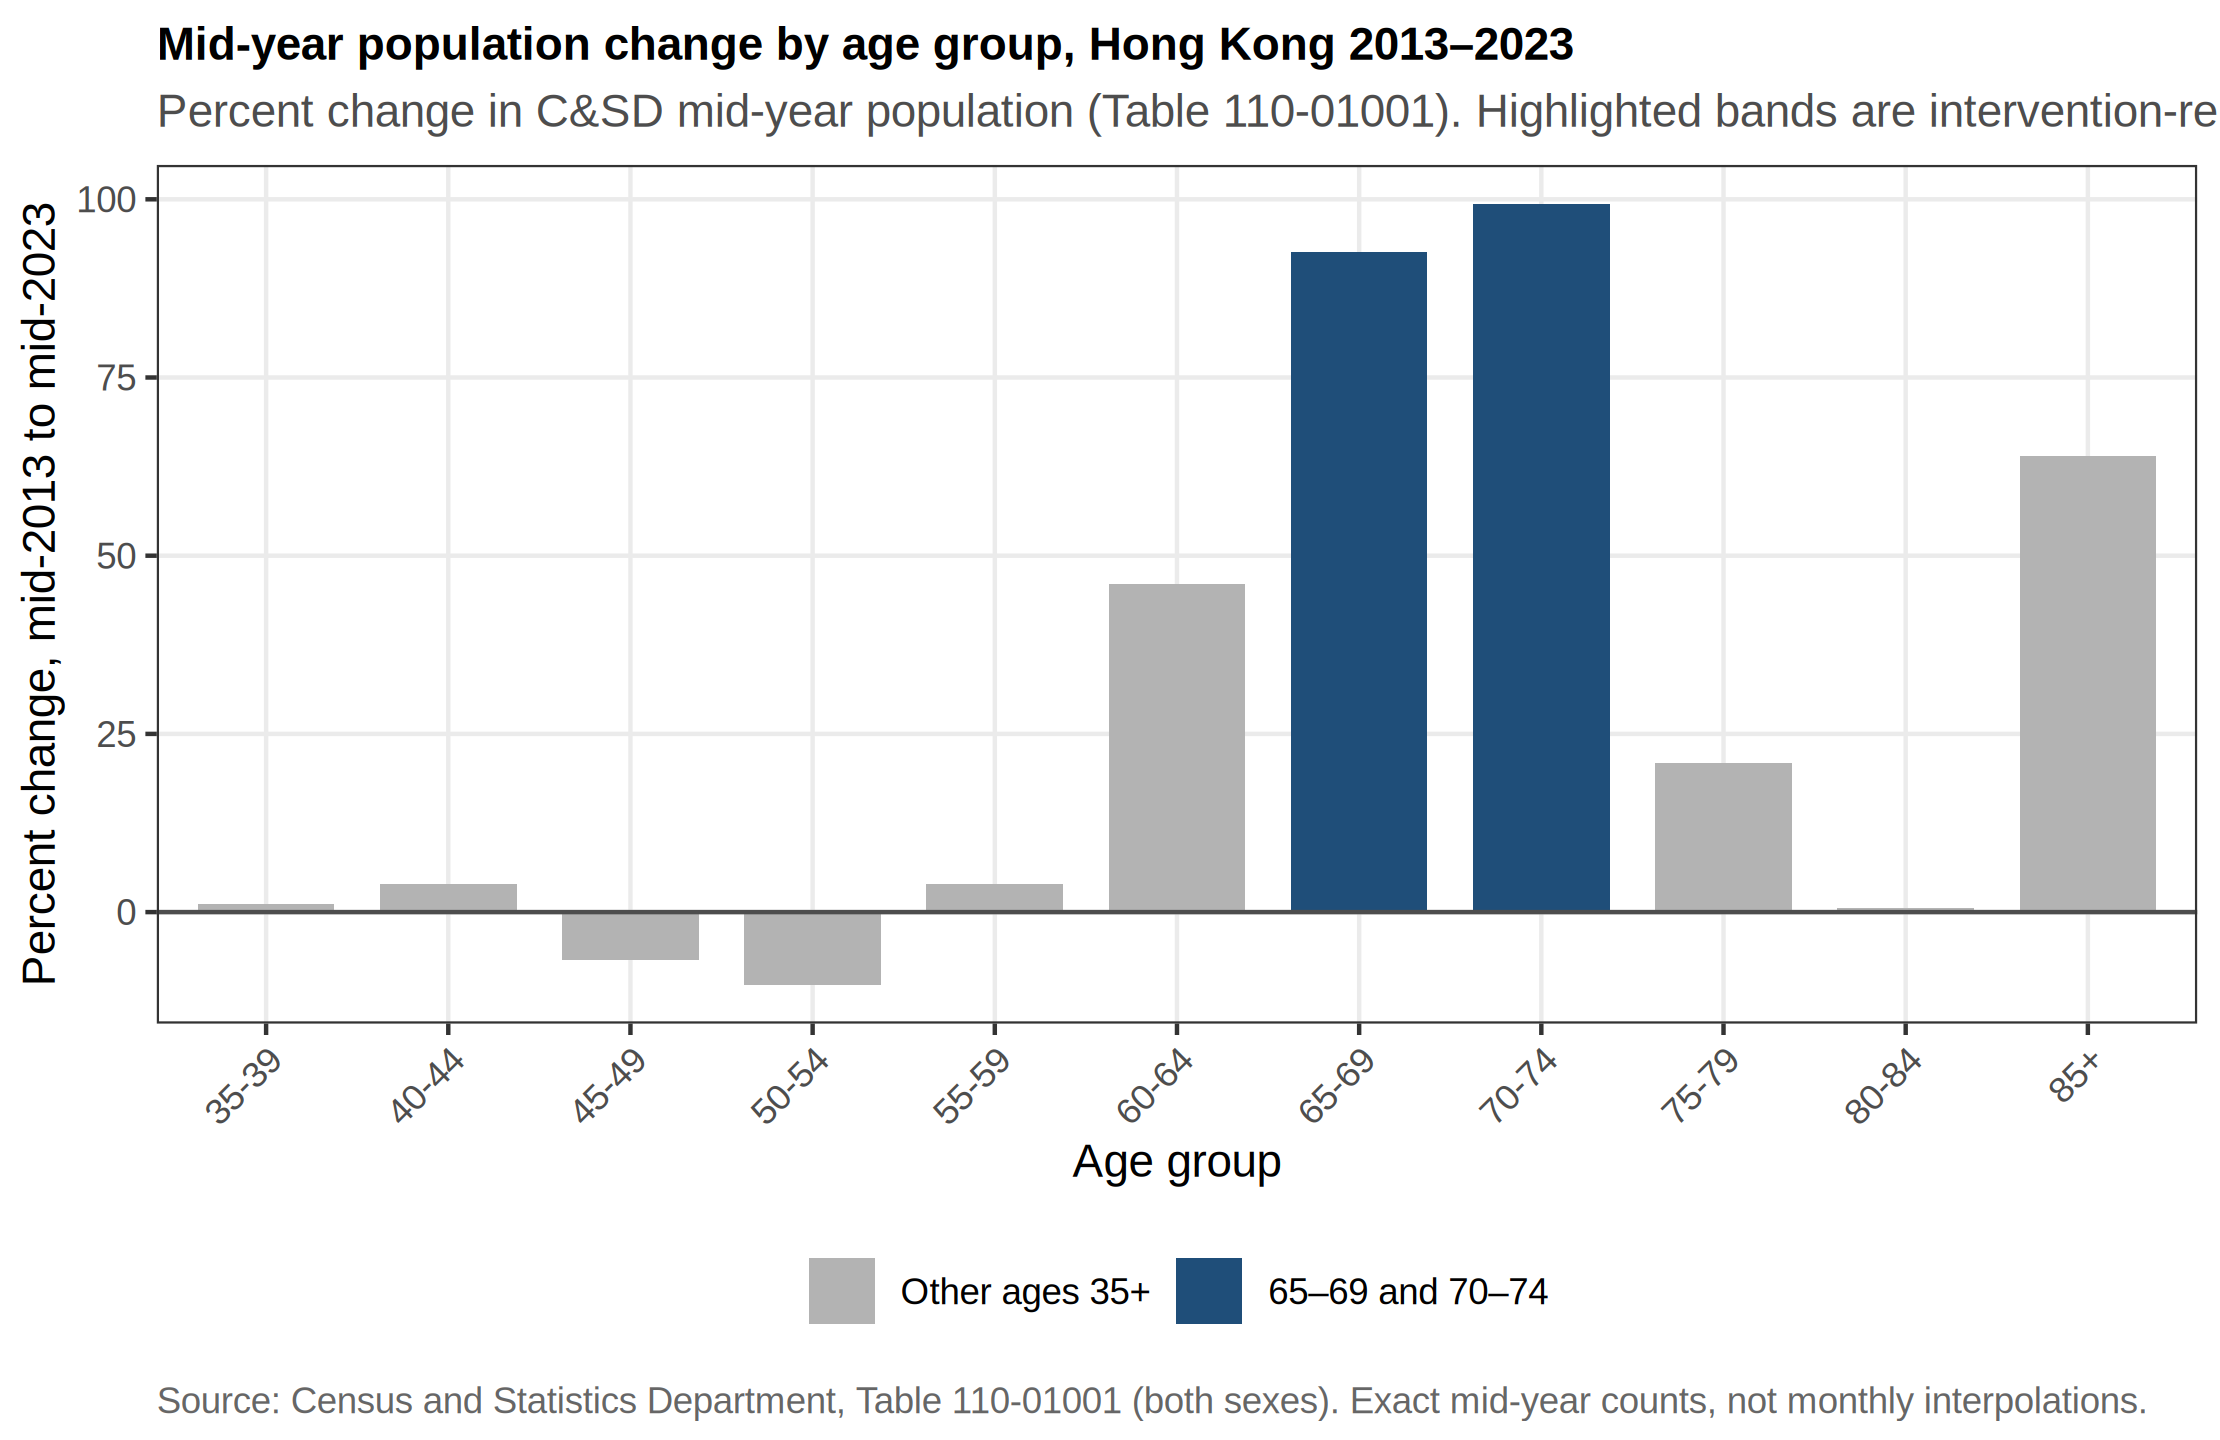
\includegraphics[width=0.88\linewidth,height=9.2cm,keepaspectratio]{../../figures/exposure_aging/fig04_population_aging_pct_change.png}\\[1pt]
\begin{flushleft}
\begin{itemize}
  \item Ages \textbf{65--69}: +92.6\% \quad|\quad \textbf{70--74}: +99.3\% \quad|\quad 85+: +63.9\%
  \item More clinically vulnerable person-time under a warming subtropical climate
\end{itemize}
\end{flushleft}
}
\end{minipage}
\end{textblock*}

% COLUMN 3
\begin{textblock*}{36.5cm}(80.3cm,8.0cm)
\begin{minipage}[t]{36.5cm}
\posterbox{6. Seventeen analysis pathways}{%
Numbered scripts turn public weather/population inputs into validated exposures,
denominators, and (when HA arrives) admission models. Dev track: synthetic HA dry-runs only.
Real track refuses synthetic outcomes.
\vspace{0.1em}
{\fontsize{9.8}{11.8}\selectfont
\renewcommand{\arraystretch}{0.98}
\begin{tabularx}{\linewidth}{@{}c>{\RaggedRight\arraybackslash}X@{\hspace{1pt}}c@{}}
\toprule
\textbf{\#} & \textbf{Pathway} & \textbf{Status} \\
\midrule
00 & Project setup \& session info & Done \\
01 & Import HKO daily weather & Done \\
02 & Build monthly climate extremes & Done \\
03 & Import / document EPD pollution & Ready \\
04 & Build monthly pollution panel & Ready \\
05 & Build C\&SD age--sex denominators & Done \\
06 & Confounders (COVID, holidays) & Done \\
07 & Synthetic HA dry-run outcomes & Dev only \\
08 & Merge analysis panel (dev) & Done \\
08b & Merge approved HA panel & Pending \\
09 & Descriptive tables & Done \\
10 & Exploratory figures & Done \\
11 & Fit NB models (syn./real) & Scaffold \\
12 & Model diagnostics & Scaffold \\
13 & Report outputs \& status & Done \\
14 & Validated extremes figure & Done \\
15 & Smoke checks (HKO 33/33) & Done \\
16 & Exposure--aging deliverable & Done \\
17 & Lab-meeting temp figures & Done \\
\bottomrule
\end{tabularx}
}
\vspace{0.15em}
{\color{Muted}\fontsize{8.5}{10}\selectfont
Dev entry: \textsf{run\_pipeline\_dev.R}\\
Real entry: \textsf{run\_pipeline\_real.R}\\
Labels: REAL / PLACEHOLDER / SYNTHETIC.\par}
}

\posterbox{7. Planned hospital-burden analysis}{%
Once HA access is live (ICD-9; patient-level admissions;
ages 65--69 \& 70--74 separable):
\begin{itemize}
  \item Aggregate to month $\times$ age $\times$ sex $\times$ diagnosis
  \item Negative-binomial rates; $\log$(population $\times$ days) offset
  \item Hot nights \& cold days (per 5 extreme days); Tmax/Tmin + lag
  \item Adjust for seasonality, trend, COVID phases; stage pollution
  \item Outcomes: AMI, ischemic stroke, hemorrhagic stroke
\end{itemize}
{\color{Warn}\bfseries\fontsize{10}{12}\selectfont
No synthetic model coefficients are presented as findings.\par}
}
\end{minipage}
\end{textblock*}

% BOTTOM LEFT: takeaways + figures
\begin{textblock*}{76.5cm}(1.8cm,61.0cm)
\begin{minipage}[t]{76.5cm}
\posterbox{8. Take-home messages}{%
\begin{enumerate}
  \item \textbf{Climate is already changing Hong Kong's thermal environment:}
        hot nights and very hot days rose sharply after 2018, while cold days did not disappear.
  \item \textbf{Humans in the pathway:} the near-doubling of ages 65--74 multiplies
        person-time at cardiovascular risk under heat and cold stress.
  \item \textbf{A reproducible 17-step analysis platform} is ready to merge official extremes
        with HA admission counts for transparent hospital-burden estimation.
\end{enumerate}
\vspace{0.15em}
\begin{minipage}[t]{0.48\linewidth}
\centering
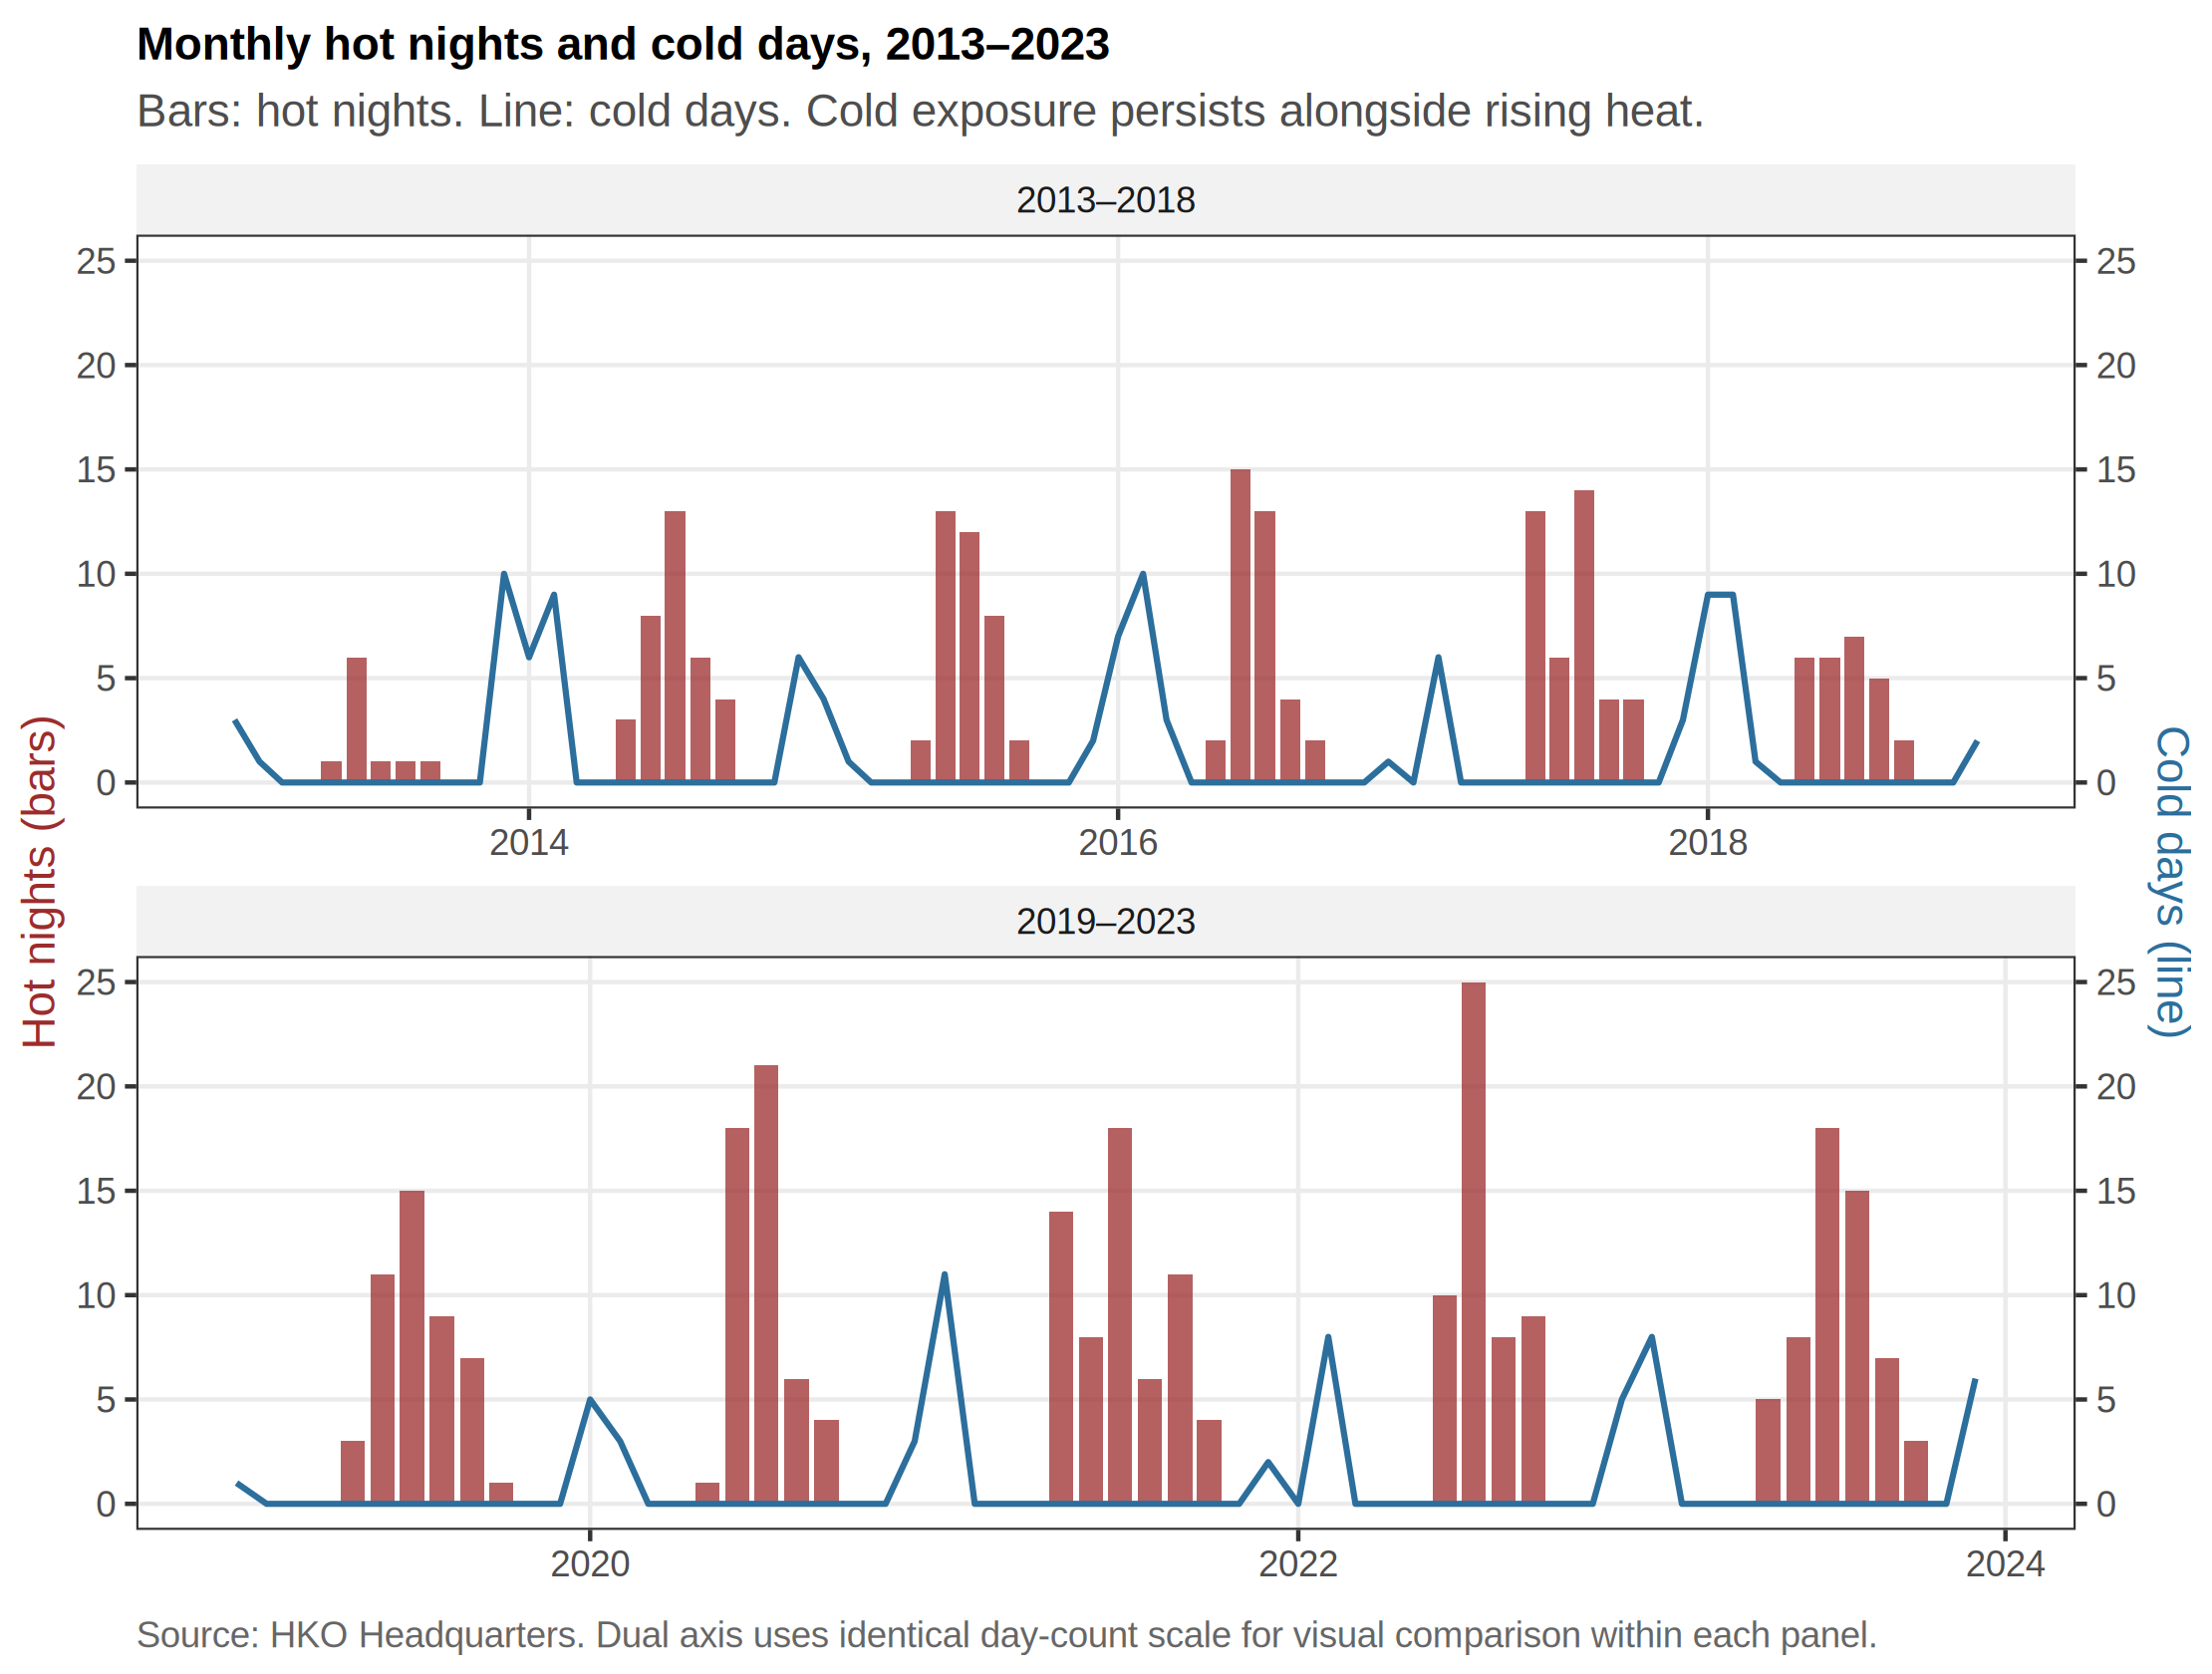
\includegraphics[width=\linewidth,height=7.2cm,keepaspectratio]{../../figures/exposure_aging/fig02_monthly_hot_nights_cold_days.png}\\[1pt]
{\color{Muted}\fontsize{8.5}{10}\selectfont Monthly hot nights (bars) vs cold days (line).\par}
\end{minipage}\hfill
\begin{minipage}[t]{0.48\linewidth}
\centering
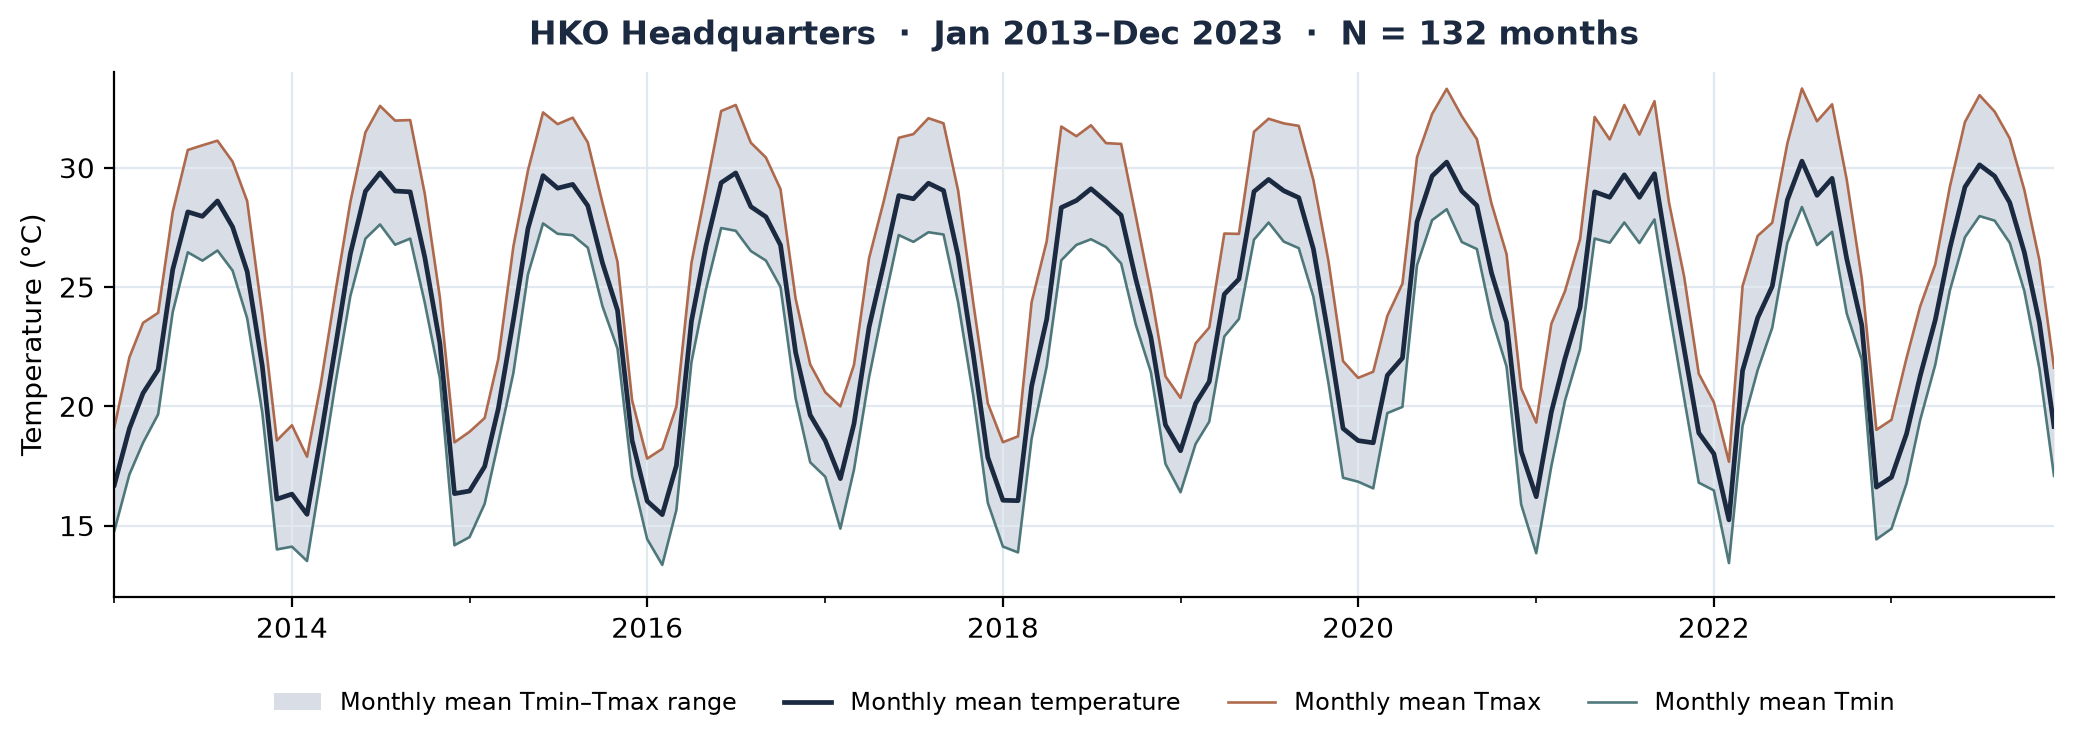
\includegraphics[width=\linewidth,height=7.2cm,keepaspectratio]{../../figures/lab_meeting/monthly_temp_ribbon_2013_2023_final.png}\\[1pt]
{\color{Muted}\fontsize{8.5}{10}\selectfont Monthly mean Tmin--Tmax ribbon ($N=132$).\par}
\end{minipage}
}
\end{minipage}
\end{textblock*}

% BOTTOM RIGHT: key numbers
\begin{textblock*}{36.5cm}(80.3cm,61.0cm)
\begin{minipage}[t]{36.5cm}
\posterbox{9. Key numbers at a glance}{%
\statchip{10$\rightarrow$61}{Hot nights/year (2013 $\rightarrow$ 2021)}
\statchip{30.7$\rightarrow$53.0}{Mean hot nights/year (2013--18 vs 2019--23)}
\statchip{+93\% / +99\%}{Population ages 65--69 / 70--74}
\statchip{33/33}{HKO Year's Weather validation matches}
\statchip{132 months}{Core window: Jan 2013--Dec 2023}
\vspace{0.15em}
{\fontsize{10.5}{13}\selectfont
\textbf{Next step:} HPC onboarding $\rightarrow$ HA QC \& Table~1 $\rightarrow$ pre-specified NB models.\\[0.2em]
\textbf{Contact:} shenrll@connect.hku.hk\\
School of Public Health, The University of Hong Kong\\[0.1em]
{\color{Muted}GEST-2026 $\cdot$ Poster $\cdot$ Environmental Toxicology and Human Health}
}
}
\end{minipage}
\end{textblock*}

\end{document}
